%%%%%%%%%%%%%%%%%%%%%%%%%%%%%%%%%%%%%%%%%%%%%%%%%%%%%%%%%%%%%%%%%%%%%%%%%%%%%%%%
% data_set.tex:
%%%%%%%%%%%%%%%%%%%%%%%%%%%%%%%%%%%%%%%%%%%%%%%%%%%%%%%%%%%%%%%%%%%%%%%%%%%%%%%%
\chapter{Background Estimation}
\label{sec:backgroundEstimation}
%%%%%%%%%%%%%%%%%%%%%%%%%%%%%%%%%%%%%%%%%%%%%%%%%%%%%%%%%%%%%%%%%%%%%%%%%%%%%%%%
The online and offline event selection criteria were applied to the data to select events where two leptons and jets were 
reconstructed, and had kinematics consistent with the \WR decay progeny.  However, these criteria also selected data events 
produced by ST background interactions, like $\DY$+jets.  The contributions of ST backgrounds to the $\Mlljj$ distribution 
found in the data were predicted using Monte Carlo (\MC) simulations and control regions with no \WR signal contamination.  
The magnitudes of the individual backgrounds, how the backgrounds were simulated, and how the control regions were defined 
and used is described here.

The magnitude of the background produced by each ST interaction is proportional to its cross section $\times$ branching ratio 
to $\ell\ell jj$ final states at $\sqrt{s} =$ 13 $\TeV$.  The \DY interaction (Figure \ref{fig:dyDiags}) produced two same flavor 
leptons with a cross section $\times$ branching ratio that peaked at 6000 pb for dilepton mass $\Mll \approx 90$ $\GeV$, 
and decreased for higher $\Mll$.  At $\sqrt{s} = 13$ $\TeV$ either quark that initiates the \DY interaction 
radiates a parton with a probability of $\sim$0.1, equal to the QCD coupling $\alpha_{QCD}$.  In $\alpha_{QCD}^{2} \sim$
0.01 $=$1\% of \DY interactions the initial quarks radiate two partons before interacting, and those partons hadronize into 
jets.  Therefore, the \DY interaction produces $\ell\ell jj$ final states with a cross section $\times$ branching ratio $\approx$ 
60 pb.  Unlike \DY, the $t\bar{t}$ quark interaction (Figure \ref{fig:ttbarDiag}) produced $\ell\ell jj$ final states without 
initial state parton radiation.  Its cross section $\times$ branching ratio, 86 pb, is similar to the cross section $\times$ 
branching ratio of \DY+2 jets.  More than 99\% of top quarks decay to a $W$ boson and bottom quark, so single top quark+$W$ boson 
interactions (Figure \ref{fig:singleTopDiags}) produced two leptons and one jet when both $W$ bosons decayed 
leptonically.  The gluon that initiates the top+W interaction radiates a gluon with $\sim$100\% probability, so the top+W interaction 
produced two lepton and two jet final states with a cross section $\times$ branching ratio of $\sim$7 pb.  Other single top quark 
interactions (Figure \ref{fig:singleTopDiags}) produce only one $W$, and therefore did not produce $\ell\ell jj$ final states 
at leading order in the electroweak coupling.  The only other interactions that produce two 
leptons and jets without initial state parton radiation are the WZ and ZZ interactions.  The WZ interaction produces two leptons and 
jets when the $W$ decays hadronically, and the $Z$ decays to charged leptons.  The ZZ interaction produces two leptons and jets 
when one $Z$ decays hadronically, and the other decays to charged leptons.  The combined WZ and ZZ interactions produced $\ell\ell jj$ 
final states with a cross section $\times$ branching ratio of $\sim$3 pb, negligible compared to the $\DY$+jets 
and $t\bar{t}$ backgrounds.  The WW interaction produces two charged leptons when both $W$ bosons decay leptonically.  The two 
quarks that initiate the WW interaction radiate two partons with $\sim$1\% probability, so the WW interaction produced $\ell\ell jj$ 
final states with a cross section $\times$ branching ratio of $\sim$0.1 pb, negligible compared to other backgrounds.  Although 
the $W$+jets and QCD multi-jet interactions do not produce $\ell\ell$ final states at leading order in the electroweak coupling, 
a small fraction of their jets, less than 0.1\%, were incorrectly reconstructed as charged leptons.  Since the $W$+jets and QCD 
multi-jet interactions produced multiple jets with large cross sections $\times$ branching ratios - in excess of several hundred pb 
\cite{wJetsMeas,jetProductionMeas} - they contributed to the $\Mlljj$ distribution found in data, but at a negligible level.  
In conclusion, the $\DY$+jets and top quark interactions produced the largest backgrounds, and other interactions produced significantly 
smaller backgrounds.  The shape and magnitude of the $\Mlljj$ distribution produced by these interactions was estimated using 
Monte Carlo (\MC) simulations.

\clearpage

\begin{figure}
	\centering
	\begin{subfigure}[t]{2.4in}
		\centering
		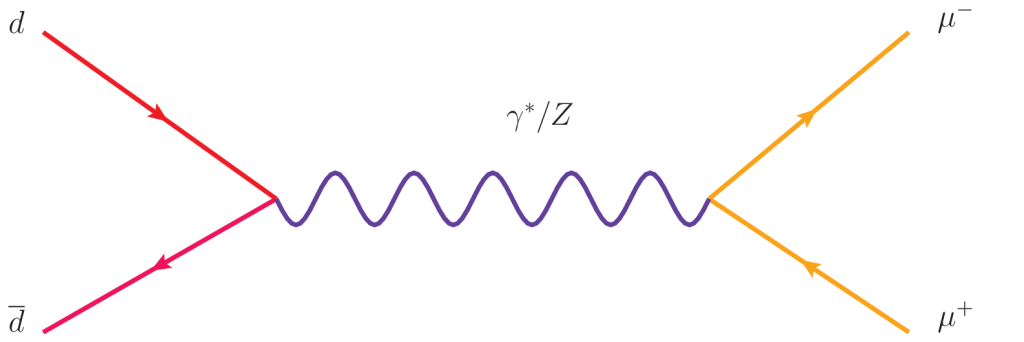
\includegraphics[width=2.4in]{figures/dyNoJetFeynDiagram.png}
	\end{subfigure}
	\thickspace
	\begin{subfigure}[t]{2.4in}
		\centering
		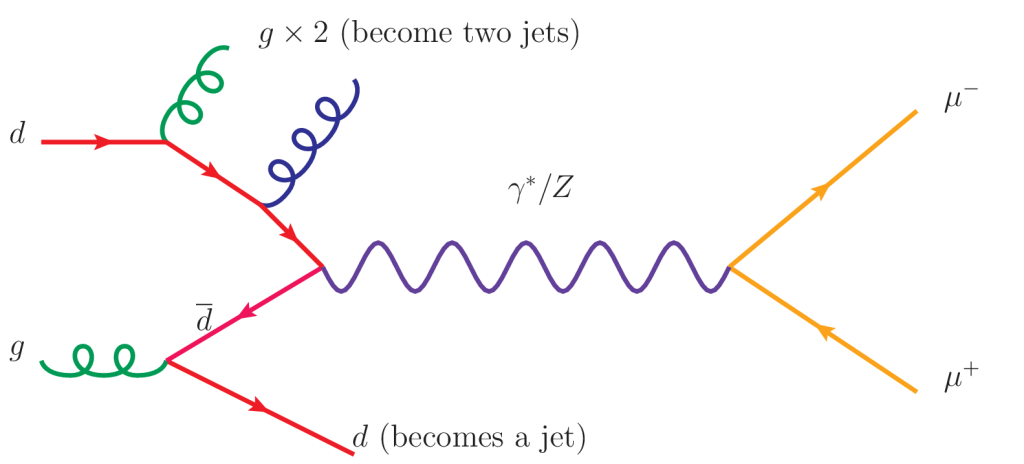
\includegraphics[width=2.4in]{figures/dyThreeJetFeynDiagram.png}
	\end{subfigure}
	\caption{Feynman diagrams for the \DY interaction with 0 radiated partons, and 3 radiated partons \cite{dyDiagrams}.}
	\label{fig:dyDiags}
\end{figure}

\begin{figure}[h]
	\centering
	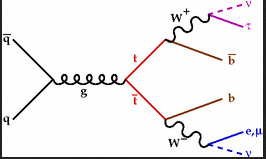
\includegraphics[width=0.45\textwidth]{figures/topAntiTopFeynDiagram.png}
	\caption{$t\bar{t}$ Feynman diagram \cite{ttbarDiagram}.}
	\label{fig:ttbarDiag}
\end{figure}

\begin{figure}[h]
	\centering
	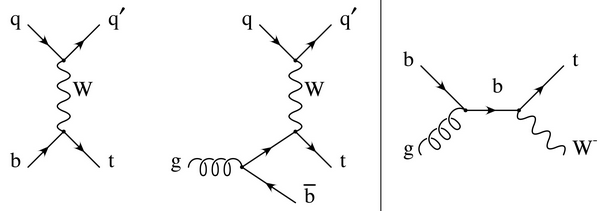
\includegraphics[width=0.7\textwidth]{figures/singleTopQuarkFeynDiagrams.png}
	\caption{Single top quark Feynman diagrams \cite{singleTopQrkDiagrams}.}
	\label{fig:singleTopDiags}
\end{figure}

\clearpage

\section{Monte Carlo}
\label{sec:MC}
Background interactions are simulated in three steps.  The first step uses one or two \MC generators to simulate the interaction between 
colliding protons, the decay of unstable particles, and the hadronization of partons leaving the interaction.  Particles produced by the 
interaction interact with the sub-detectors, and the signals generated in the sub-detectors are simulated in the second step.  In the third 
step, the reconstruction algorithms process the simulated signals to reconstruct leptons and jets.

In the first step, one \MC generator simulates the interaction between colliding protons, and the decay of unstable particles.  
The \MC generator used to simulate the background was chosen such that the strengths of the generator matched the characteristics of the 
interaction.  The \MADGRAPH generator \cite{madgraph} simulates all Feynman diagrams of a interaction at leading order in the electroweak 
coupling with up to 4 additional partons radiated from the interaction.  Due to the $\alpha_{QCD}$ cross section penalty of radiating an 
additional parton, simulating up to 4 radiated partons was only warranted for high cross section $\times$ branching ratio interactions - \DY, 
$t\bar{t} \rightarrow \ell\ell jj$, and $W \rightarrow \ell\nu$.  Therefore, \MADGRAPH was used to simulate the $\DY$+jets, $t\bar{t}$ 
and $W$+jets interactions.  In contrast with \MADGRAPH, the \POWHEG generator \cite{powheg} simulated all Feynman diagrams of a 
interaction at next-to-leading order in the electroweak and QCD couplings with up to one additional parton radiated from the interaction.  
\POWHEG was used to simulate single top quark interactions because their cross sections $\times$ branching ratios to $\ell\ell jj$ 
final states are at least 7\% larger at next-to-leading order relative to leading order \cite{singleTopNLOvsLO}.  
Although the next-to-leading order correction to the diboson (WW, WZ, ZZ) cross section $\times$ branching ratio was up to 45\% 
\cite{dibosonLOvsNLO}, the diboson background at any order is still negligible compared to the $\DY$+jets and top quark backgrounds.  Therefore, 
the production and decay of diboson pairs was simulated using the leading order \PYTHIA generator \cite{pythia8,Sjostrand:2006za}, 
with up to one additional parton radiated from the interaction.  Electroweak and QCD interactions simulated with any \MC generator show 
the best agreement with experimental data when \PYTHIA is used to simulate parton hadronization \cite{pythiaForHadronization}, so all 
simulations used \PYTHIA and the NNPDF23 PDF set \cite{nnpdf} to simulate parton hadronization.  Excluding the partons, the \MC generator 
that simulated the pp interaction also simulated the decay of unstable particles to quasi-stable and stable particles, like the $\Sigma^{\pm}$ 
and $\gamma$, that travel a mean distance c$\tau \gtrsim 2.4$ cm before decaying.  Particles that travel a mean distance of 2.4 cm have a 
small probability to interact with the first silicon pixel tracker layer located 4.4 cm from the interaction point \cite{cmsTdrPhysPerformance}, 
so they are not decayed before the detector response is simulated.

%SAVE THIS statement that explains why the aMCatNLO inclusive diboson simulated datasets were not used
%A second set of diboson$\to$leptons+jets events was simulated with a next-to-leading order \MC generator, but these events were 
%generated with positive and negative event weights.  Due to the presence of positive and negative event weights, in some $\Mlljj$ 
%regions the predicted number of diboson events was negative, and the prediction's statistical uncertainty was greater than 100\%.

In the second step, the effect of pileup is simulated, and GEANT \cite{geant4} simulates the propagation and decay of quasi-stable and stable 
particles, and their interactions with the detector.  The large instantaneous luminosity of the LHC beams produced multiple pp interactions 
(pileup) in each event in data.  When \MC simulations started in the spring of 2015, the pileup distribution found in data was expected to 
follow a Poisson distribution with mean 12.  In each simulated event, the effect of pileup is simulated by pulling a 
random integer $X$ from a Poisson distribution with mean 12, and mixing $X$ simulated minimum bias events into the event.  The 
minimum bias events were simulated only through the first simulation step.  The distributions of reconstructed particle multiplicity and 
kinematics found in minimum bias events in data show the best agreement with those found in events simulated with \PYTHIA 
\cite{pythiaForHadronization}, so \PYTHIA was used to simulate minimum bias events.  After adding minimum bias events, GEANT propagates all 
particles (stable and quasi-stable) through the 3.8 $\unit{T}$ magnetic field, simulates their interactions with the detector and the resulting 
signals, and simulates the decays of quasi-stable particles to the following stable particles - $\gamma,p^{\pm},n^{0},\bar{n}^{0},\nu,e^{\pm}$.

In the third step, particle reconstruction algorithms reconstruct particles and vertices at the trigger level and offline using the detector 
signals simulated by GEANT.  The trigger selections are applied, and the final decision of each trigger algorithm, pass or fail, is saved in each 
simulated event, but no events are discarded.

After the third step, particle energy corrections and event weights are applied.  As explained previously, the energies of simulated jets, muons, 
and electrons were corrected to match the energy of particles reconstructed in data.  The differences in lepton reconstruction, trigger selection, 
and offline ID selection efficiencies between data and simulated events were corrected by changing the weight of each simulated event, up to 
$\pm$7\%, depending on the $\pt$ and $\eta$ of the selected leptons.  Independent of the kinematics of reconstructed particles, the weight of each 
simulated event was normalized to the integrated luminosity of the data, and adjusted further to match the pileup distribution found in the data.  The 
simulated pileup distribution is a Poisson distribution with mean 12, but the pileup distribution found in the data is better represented by a Poisson 
distribution with mean 14 \cite{lumi}.  The discrepancy between the data and simulated pileup distributions was corrected by changing the weight of 
each simulated event, on average by $\sim$5\%.

The simulated interactions are summarized in Table \ref{tab:centrallyProducedMC}.  The number of simulated events for each interaction is expressed 
in units of fb$^{-1}$, and should be compared to the 2.6 fb$^{-1}$ of data that was collected.

\begin{table}[bt]
	\caption{The ST background and \WR signal (only $\mnul = \frac{1}{2}\mWR$) simulated datasets.  The "Size" of a dataset is equal 
	to the number of simulated events divided by the 13 $\TeV$ cross section $\times$ branching ratio of the process.}
\label{tab:centrallyProducedMC}

\centering
\resizebox{\textwidth}{!}{
	\begin{tabular}{ |c|c|c|c| } 
	\hline
	Dataset         & Step 1 Generator & cross section (pb) & Size (fb$^{-1}$)   \\
		\hline
		Inclusive DY+jets, $DY \rightarrow ll$ & \MADGRAPH   & 5991    & 1.51 \\ \hline
		DY+jets HT 100-200, $DY \rightarrow ll$ & \MADGRAPH   & 181.3    & 15.0 \\ \hline
		DY+jets HT 200-400, $DY \rightarrow ll$ & \MADGRAPH   & 50.42    & 19.3 \\ \hline
		DY+jets HT 400-600, $DY \rightarrow ll$ & \MADGRAPH   & 6.984    & 153. \\ \hline
		DY+jets HT $>$ 600, $DY \rightarrow ll$ & \MADGRAPH   & 2.704    & 369. \\ \hline
		t$\bar{t}$+jets $\rightarrow ll$+jets & \MADGRAPH  & 85.67    & 286. \\ \hline
		single t $\rightarrow$ leptons+jets  & \POWHEG & 80.95 & 20.8 \\ \hline
		single $\bar{t}$ $\rightarrow$ leptons+jets & \POWHEG & 136.0 & 24.3 \\ \hline
		$\bar{t}$+W $\rightarrow$ all   & \POWHEG & 35.85 & 27.6 \\ \hline
		t+W $\rightarrow$ all   & \POWHEG & 35.85 & 27.8 \\ \hline
		WW $\rightarrow$ all  & \PYTHIA & 113.8   & 8.73   \\ \hline
		ZZ $\rightarrow$ all  & \PYTHIA & 10.15   & 98.2   \\ \hline
		WZ $\rightarrow$ all  & \PYTHIA & 23.4   & 41.8   \\ \hline
		W+jets $\rightarrow l\nu$+jets & \MADGRAPH & 50270   & 1.44 \\ \hline
		%$\WR \rightarrow l\nul \rightarrow lljj$  & \PYTHIA & 1$\times 10^{-5}$ - 4.3 & 5$\times 10^{6}$ - 11.6   \\ \hline
		\end{tabular}
}
\end{table}


\section{Top Quark Background}
\label{sec:topQrkBkgnds}
Top quark interactions, primarily those that produce a $t\bar{t}$ pair, produce bottom quarks and gluons that hadronize into jets, and 
two $W$ bosons that yield two charged leptons.  Since $W$ bosons decay to electrons and muons with equal branching ratios, top quark 
interactions produce the $e\mu jj$ final state twice as often as the $eejj$ or $\mu\mu jj$ final states.  Since the $e\mu jj$ final state 
is not contaminated with \WR signal (Chapter \ref{sec:lrsPhenomenology}) or other background interactions, the $e\mu jj$ final state was 
used as a control region to estimate the top quark background.  During collisions, $e\mu jj$ events were selected using the Level-1 single 
muon trigger described in Chapter \ref{sec:onlineAndOfflineIdSel}.  Then, events were selected using the following 
$e\mu$ HLT selection criteria:

\begin{itemize}
	\item A track reconstructed in the silicon tracker with $\pt > 30$ $\GeV$ and $|\eta| < 2.4$ was geometrically matched to 
		the muon detector track segment that passed the L1 trigger.
	\item In the plane perpendicular to the beam axis, the distance between the silicon tracker track origin and its 
		reconstructed vertex was $< 1$ mm.
	\item One 5 $\times$ 5 ECAL crystal cluster was required to have $\Et > 30$ $\GeV$.
	\item For the selected ECAL cluster (energy E):
	\begin{itemize}
		\item The hadronic energy behind the cluster was $<$ 15\% of E in the barrel, and $<$ 10\% of E in the endcap. 
		\item Ninety percent of E was measured in an area that was two crystals wide in $\eta$.
		\item If the cluster was in the barrel, a reconstructed track with signals in at least two pixel tracker layers 
			extrapolated close to the cluster position.  The track extrapolated from the pixel tracker to within $2.3$ cm 
			of the cluster $z$ position, and to within 1 ECAL crystal area of the cluster $(\eta,\phi)$ position.
	\end{itemize}
\end{itemize}

In events selected by the trigger, leptons and jets were reconstructed and selected offline using the reconstruction algorithms and selection 
criteria described in Chapter \ref{sec:reco_chapter}, with the additional requirement that one selected lepton is an electron, and the other 
a muon.  The same selection criteria were applied to simulated background events, and compared to the selected data events in Figure 
\ref{fig:dataAndSimsInEMuChannel}.  Comparing the magnitudes of different simulated backgrounds, the top quark background produces more than 
98\% of selected $e\mu jj$ events, as expected.

\begin{figure}[h]
	\centering
	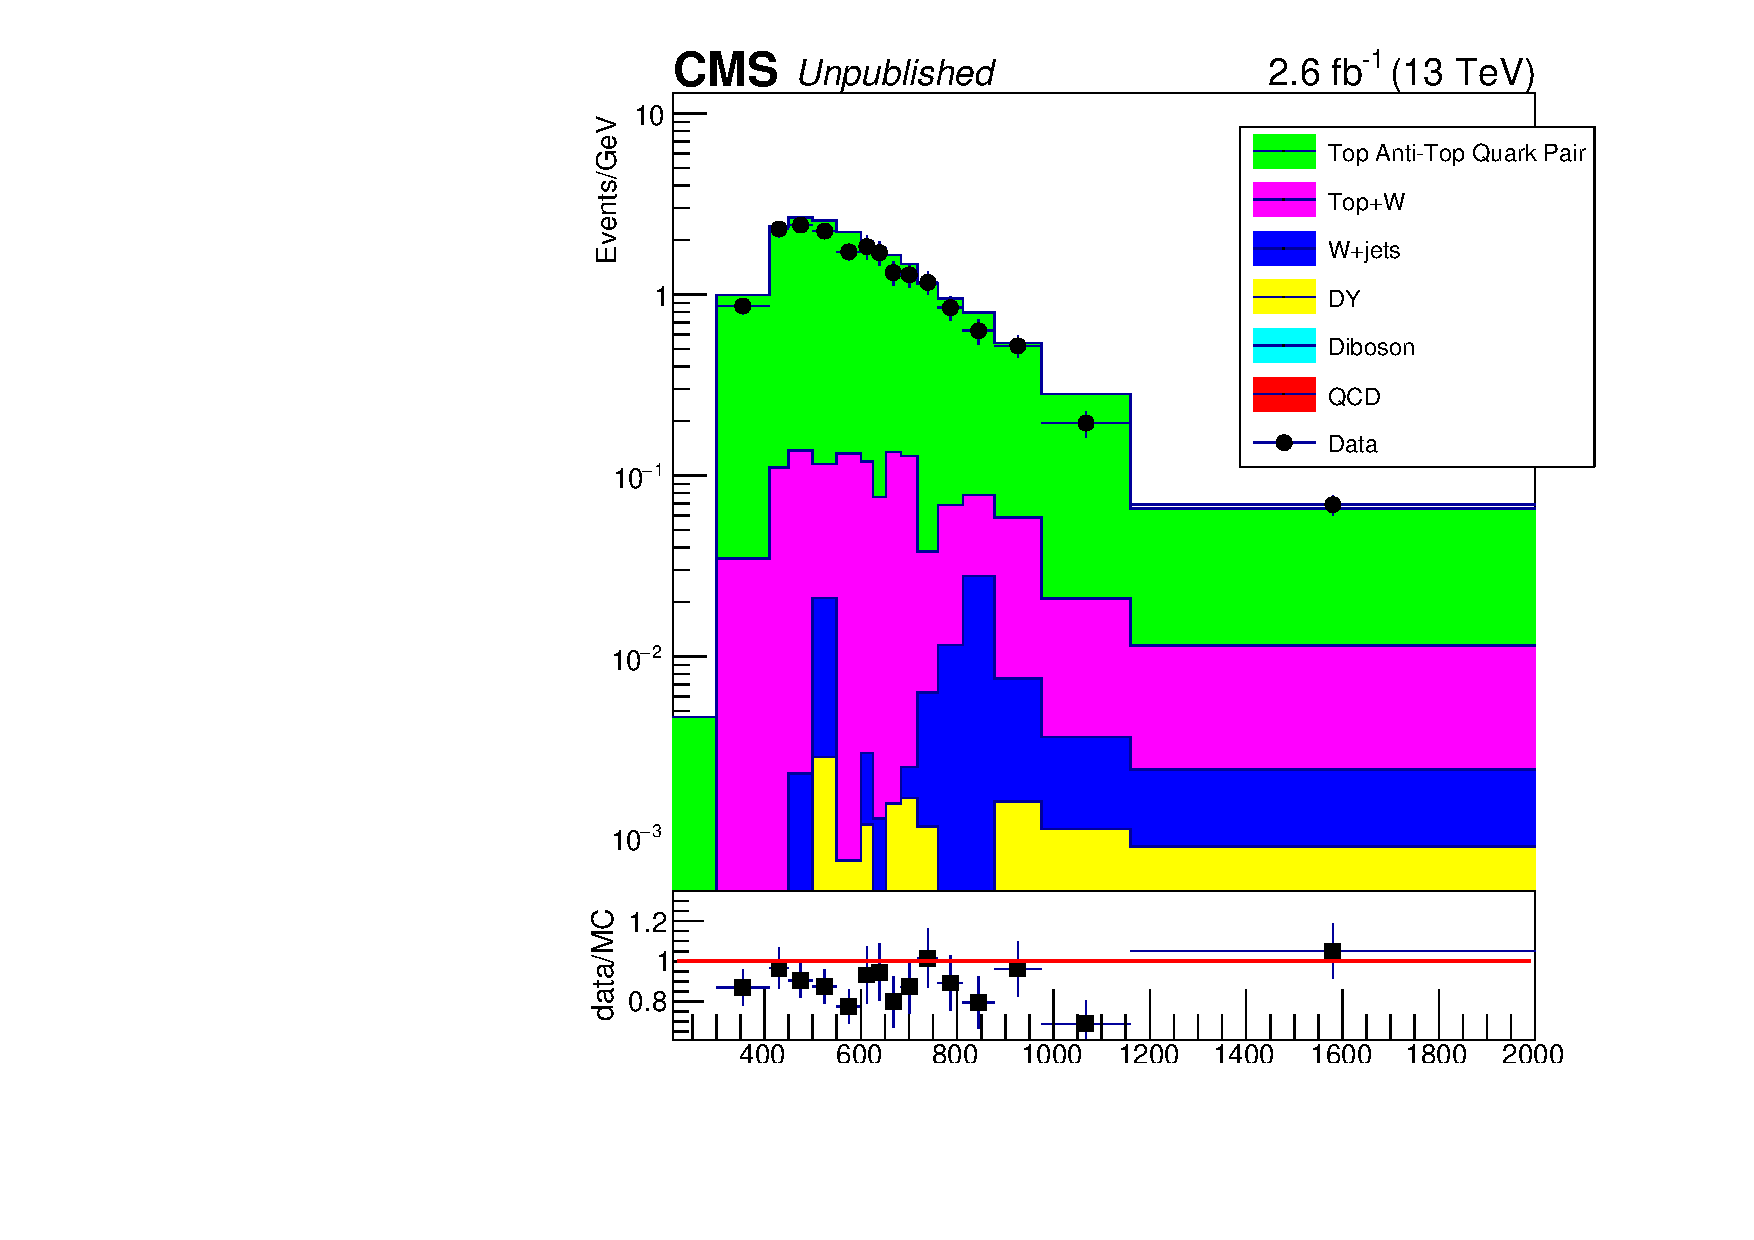
\includegraphics[width=0.7\textwidth]{figures/Mlljj_eMuChannel_log.pdf}
	\caption{The $\Mlljj$ distribution from data and simulated ST events that passed the $e\mu$ selection criteria, excluding 
	the $\Mlljj > 600 \GeV$ cut.  The bin widths were variable, and their contents were normalized to the bin widths.}
	\label{fig:dataAndSimsInEMuChannel}
\end{figure}

The $\Memujj$ distribution found in selected data events was scaled by two factors to estimate the top quark background in the $ee$- 
and $\mu\mu$-channels.  The first factor, the ratio of $\frac{\ell\ell}{e\mu}$ production, is 0.5, and is independent of $\Mlljj$.  The 
second factor, the ratio of the electron and muon selection efficiencies $\frac{e}{\mu}$, is expected to be below 1 because electrons 
reconstructed with $1.44 < |\eta| < 1.57$ are ignored.  However, the exact value of $\frac{e}{\mu}$ and its variation with $\Mlljj$ were 
not known from first principles.  The product of the two factors and the product's variation with $\Mlljj$ was estimated using 
simulated top quark events.  First, simulated events were selected using the $e\mu$-, $ee$-, and $\mu\mu$-channel selection 
criteria.  Then, the $\Mlljj$ distribution found in each set of events was split into variable width bins such that each bin had 
the same number of events.  The first bin covered $600 < \Mlljj \leq 625$ $\GeV$, and the last bin covered $\Mlljj > 1160$ $\GeV$.  
Then, the integral of each bin was calculated for all three distributions.  Finally, the integrals of the $\Meejj$ and $\Mmumujj$ bins 
were divided by the integrals of the $\Memujj$ bins.  The result, shown in Figure \ref{fig:ttbarSFratios}, represents the product of 
the $\frac{\ell\ell}{e\mu}$ production ratio and the $\frac{e}{\mu}$ (or $\frac{\mu}{e}$) selection efficiency ratio as a function of $\Mlljj$.  
The result within statistical uncertainty is consistent with a constant value versus $\Mlljj$: 0.659 for $\Mmumujj / \Memujj$, 0.432 
for $\Meejj / \Memujj$.  This confirms that the $\Mlljj$ distribution shape found in top quark events is independent of the final state 
lepton flavor.  In addition, it means that the top quark contributions to the $\Mlljj$ distributions found in data can be predicted by 
the $\Memujj$ distribution found in data multiplied by a constant.

\begin{figure}
	\centering
	\begin{subfigure}[t]{2.4in}
		\centering
		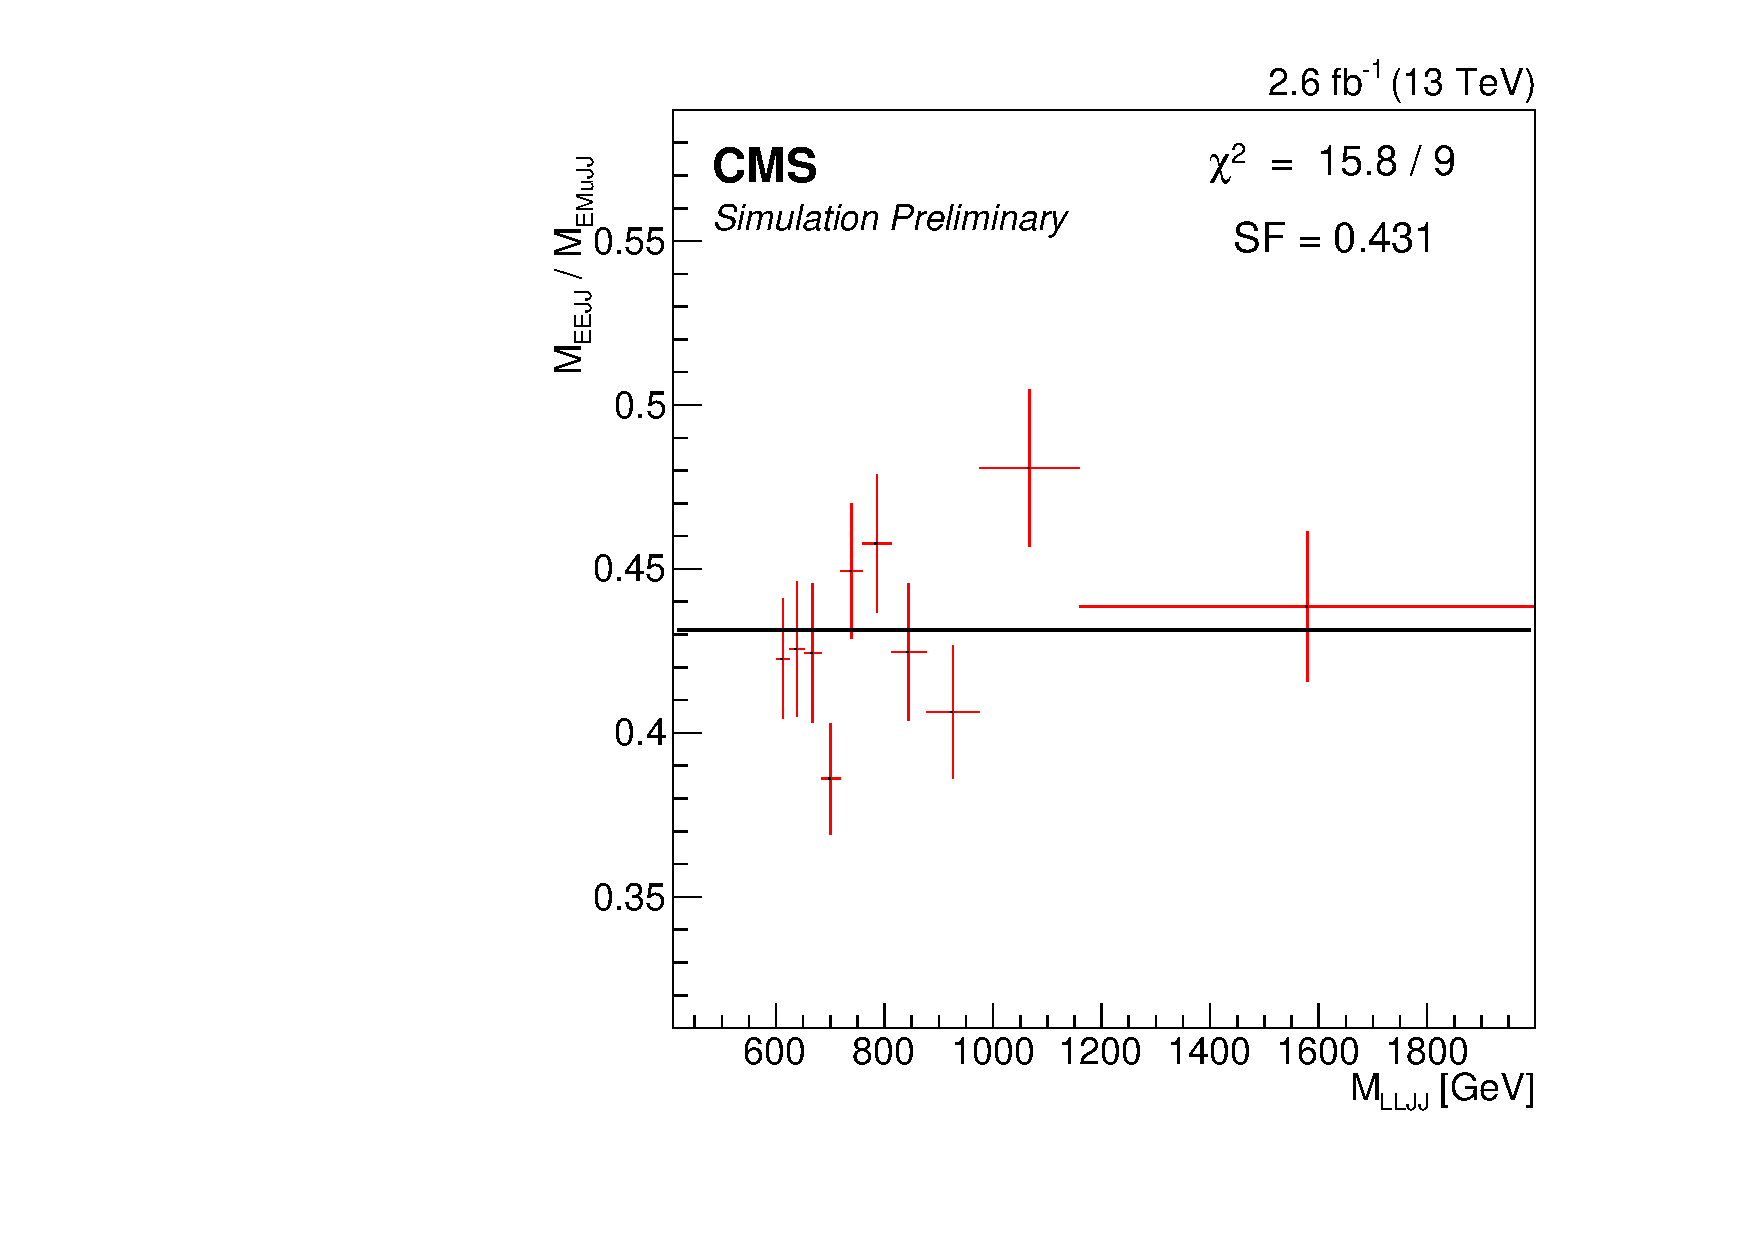
\includegraphics[width=2.4in]{figures/flavor_ratio_EE_variablebinwidth.pdf}
	\end{subfigure}
	\thickspace
	\begin{subfigure}[t]{2.4in}
		\centering
		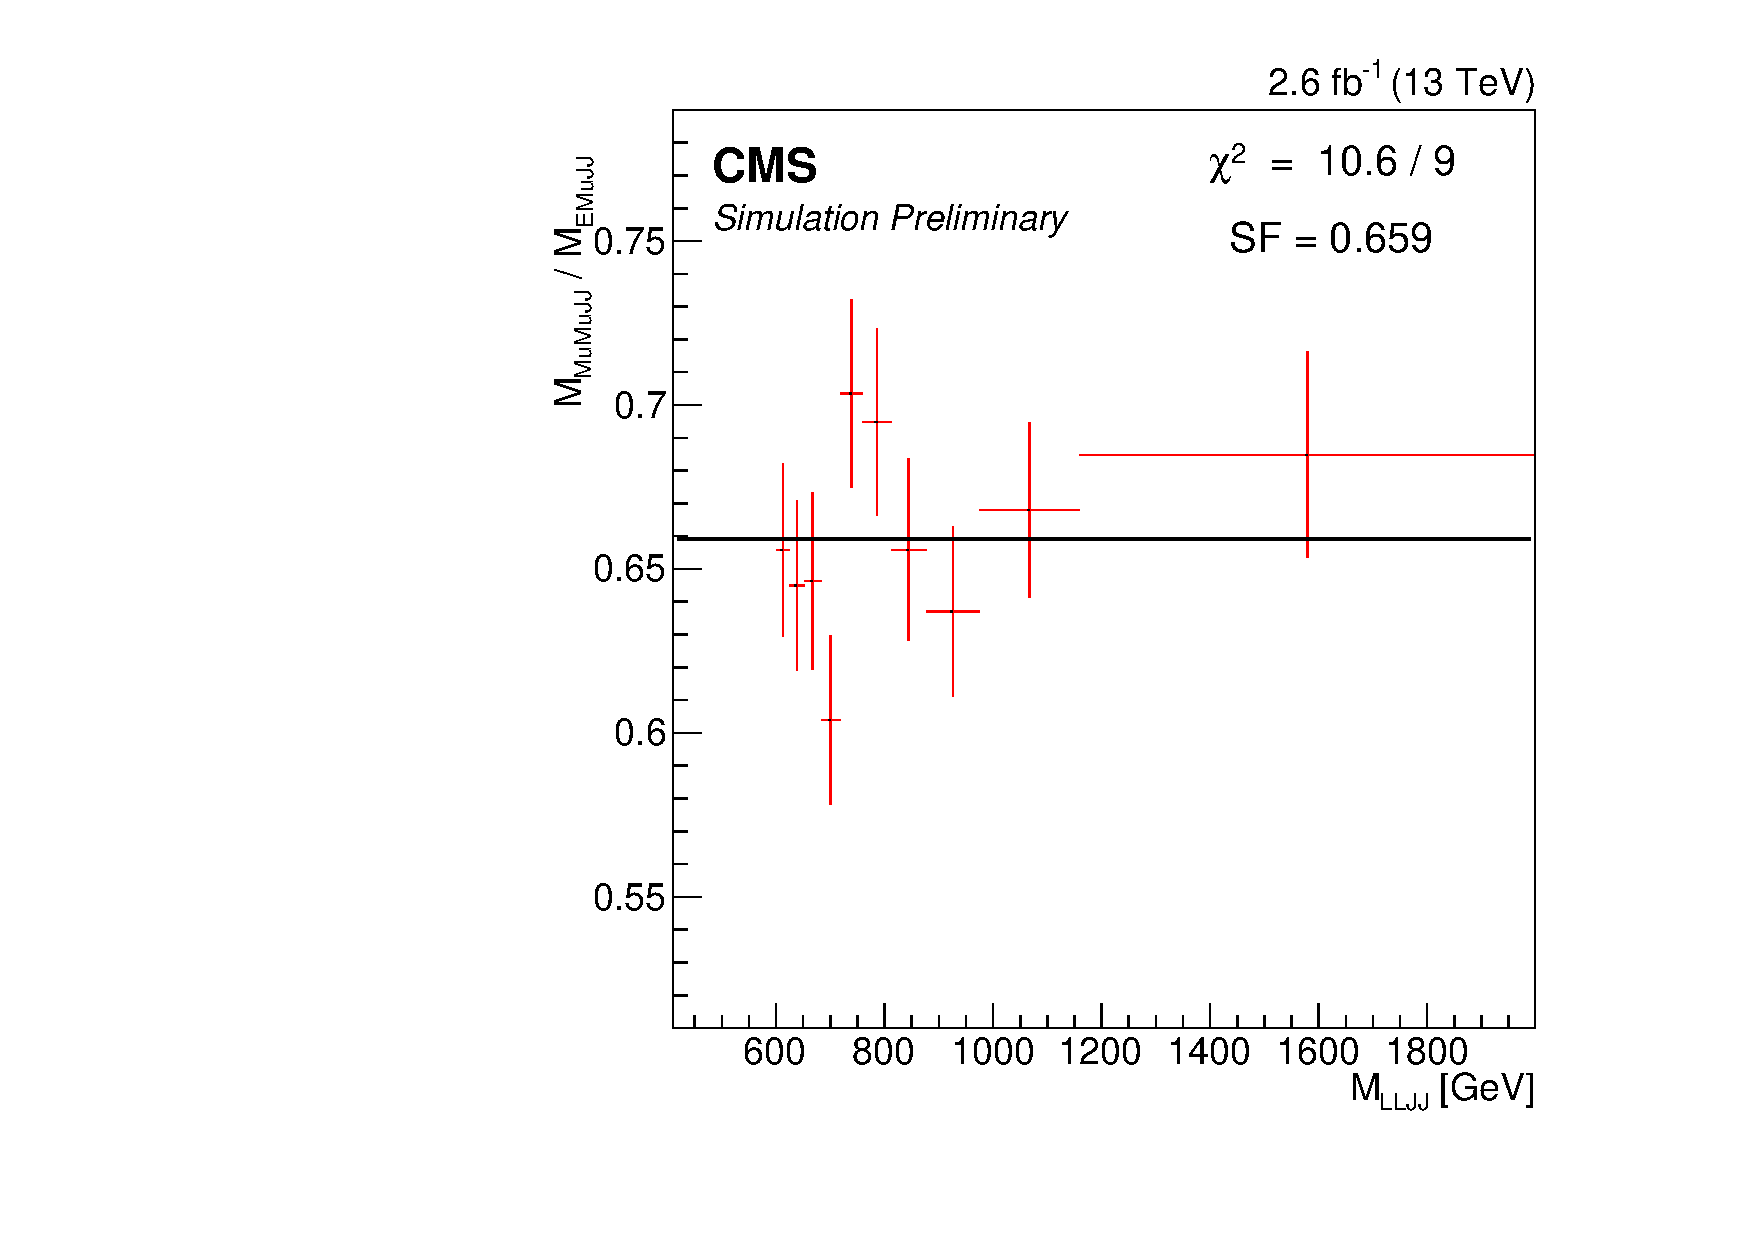
\includegraphics[width=2.4in]{figures/flavor_ratio_MuMu_variablebinwidth.pdf}
	\end{subfigure}
	\caption{The bin-by-bin ratio of the $\Mlljj$ and $\Memujj$ distributions from simulated top quark backgrounds, where 
		$\ell$ is an electron on the left, and a muon on the right.}
	\label{fig:ttbarSFratios}
\end{figure}

The $\Memujj$ distribution found in data was multiplied by 0.659 or 0.432 to estimate the top quark $\Mlljj$ distribution in the 
$\mu\mu$- or $ee$-channel.  Although the values 0.659 and 0.432 were calculated using all simulated events with $\Mlljj > 600$ $\GeV$, 
the majority of selected simulated events had $\Mlljj < 1500$ $\GeV$.  A 10\% uncertainty was assigned to the top quark background 
estimate to cover any deviation from 0.659 or 0.432 at high $\Mlljj$.  Based data and simulated events shown in Figure 
\ref{fig:dataAndSimsInEMuChannel}, the non-top quark backgrounds contributed $\sim$1\% to the $\Memujj$ distribution found in data.  
Their contribution was neglected because it was less than the 10\% top quark background uncertainty.


\section{\DY Background}
\label{sec:dyBkgnd}
The $\DY$+jets and top quark interactions produced $\ell\ell jj$ events at similar rates, much higher than other interactions.  Since 
the $\Mlljj$ distribution shape found in top quark events was the same in the $ee$-, $e\mu$-, and $\mu\mu$-channels, 
the top quark background was estimated directly from data in the $e\mu$ control region.  No analogue of the signal free $e\mu$ control region 
exists for the $\DY$+jets background, so the \DY background was estimated using simulated events.  The simulated \DY interaction is a 
simplified version of the \DY interaction that occurs in real collisions, and the effect of those simplifications was estimated by 
comparing simulated background events to data events in three control regions.

\subsection{\DY normalization in $\Mlljj$}
\label{sec:dyNormInMlljj}
Simulated $\DY$+jets events were produced at leading order in the electroweak and QCD couplings, and $\DY$+jets events found in 
data were produced at all orders in these couplings.  The difference in the coupling orders created discrepancies between data and 
simulations in the production rate and kinematics of leptons and jets.  The discrepancy in production rate was minimized by 
weighting the simulated events based on the integrated luminosity of data $\times$ the next-to-next-to-leading order \DY cross section 
$\times$ branching ratio.  The weight was the same for all simulated events, and did not correct the discrepancy in the lepton and jet 
kinematics.

The effect of the kinematic discrepancy was estimated by comparing data to simulated $\DY$+jets events in the $Z \rightarrow \ell\ell$ 
control region, where the majority of events were produced by the $\DY$+jets interaction.  Events in the $ee$-channel control region were 
selected using a Level-1 trigger that required one 5 $\times$ 5 ECAL crystal cluster with $\Et > 30$ $\GeV$ and $|\eta| < 2.1$.  Then, 
selected events were required to pass the following double-electron HLT selection criteria:

\begin{itemize}
	\item One 5 $\times$ 5 ECAL crystal cluster was required to have $\Et > 30$ $\GeV$, and a second non-overlapping cluster 
		was required to have $\Et > 4$ $\GeV$.
	\item For the cluster with $\Et > 30$ $\GeV$ (energy E):
	\begin{itemize}
		\item The hadronic energy behind the cluster was $<$ 5.5\% of E in the barrel, and $<$ 7\% of E in the endcap. 
		\item Ninety percent of E was measured in an area that was two crystals wide in $\eta$.
		\item A reconstructed track with signals in at least two pixel tracker layers extrapolated close to the cluster 
			position.  The track extrapolated from the pixel tracker to within 1 cm of the cluster $z$ position, and to 
			the cluster $(\eta,\phi)$ position within half the area of one ECAL crystal.
		\item The cluster $\Et$ and matching track $\pt$ cannot differ by more than 50\%. 
		
		\item In a $\Delta R =$ 0.3 radius cone centered on the cluster:
		\begin{itemize}
			\item The total ECAL energy not measured in the cluster was $<$ 22.5\% of E in the barrel, and $<$ 12.1\% of 
				E in the endcap.
			\item The total HCAL energy was $<$ 15.5\% of E in the barrel, and $<$ 16\% of E in the endcap.
		\end{itemize}
	\end{itemize}
\end{itemize}

Events in the $\mu\mu$-channel control region were selected using a Level-1 single muon trigger.  The Level-1 trigger was identical to 
the Level-1 single muon trigger used in the $e\mu$ control region, but required one track that had $\pt > 20$ $\GeV$.  Then, selected 
events were required to pass the following single muon HLT selection criteria:

\begin{itemize}
	\item A track reconstructed in the silicon tracker with $\pt_{1} > 22$ $\GeV$ and $|\eta| < 2.4$ was geometrically matched to 
		the muon detector track segment, reconstructed with $\pt_{2}$ that passed the L1 trigger.
	\item In the plane perpendicular to the beam axis, the distance between the silicon tracker track origin and its 
		reconstructed vertex was $< 1$ mm.
	\item In a $\Delta R =$ 0.3 radius cone centered on the muon trajectory:
		\begin{itemize}
			\item The total ECAL energy was $<$ 11\% of $\pt_{2}$ in the barrel, and $<$ 8\% of $\pt_{2}$ in the endcap.
			\item The total HCAL energy was $<$ 21\% of $\pt_{2}$ in the barrel, and $<$ 22\% of $\pt_{2}$ in the endcap.
			\item The total $\pt$ of all silicon tracker tracks excluding the muon track was $<$ 9\% of $\pt_{1}$.
		\end{itemize}
\end{itemize}

Electrons reconstructed in simulated events passed the trigger criteria with a different efficiency than electrons reconstructed in 
data.  The efficiency difference was corrected by multiplying the weight of every simulated event by a weight that depended on the 
$\Et$ and $\eta$ of the electron that passed the highest energy requirement.  The average weight was 0.96 (4\% decrease).  No correction 
was needed in the muon channel.

In events selected by the triggers, reconstructed leptons and jets were selected using offline selection criteria.  The ID criteria 
were identical to those described previously.  The kinematic selection criteria, listed in Table \ref{tab:cutsZllReg}, use lower lepton 
$\pt$ thresholds to select more $Z\rightarrow \ell\ell$ events.

\begin{table}[h]
	\caption{The kinematic selection criteria applied to events in the $Z\rightarrow \ell\ell$ control region 
	to select two leptons and two jets.}
	\label{tab:cutsZllReg}
	\centering
	\begin{tabular}{c|c}
		variable & criteria \\  \hline
		jet $\pt$ and $\eta$ & $\pt > 40$, $|\eta| < 2.4$ \\
		lepton-jet separation & $\Delta R > 0.4$ \\
		lepton $\pt$ and $\eta$ & $\pt > 35$, $|\eta| < 2.4$ \\
		di-lepton mass $\Mll$ & $70 < \Mll < 110$ \\
	\end{tabular}
\end{table}

The $\Mll$ distribution found in selected $Z\rightarrow \ell\ell$ events was compared between data and $\DY$+jets simulations.  Due to 
the lepton and jet kinematic discrepancy, the normalization of the $\Mll$ distribution found in data exceeded the normalization found in 
simulated events by 15.7\% in the $ee$-channel, and 14.2\% in the $\mu\mu$-channel.  The effect of the kinematic discrepancy was 
minimized by increasing the weight of simulated $\DY$+jets events by 15.7\% in the $ee$-channel, and 14.2\% in the $\mu\mu$-channel.  
The uncertainty on this normalization correction, discussed next, was comparable to the background from other interactions in the 
$Z \rightarrow \ell\ell$ control region.  As a result, the contributions of other interactions to the data in the control region were 
neglected.

Two additional $\DY$+jets datasets were simulated using different generators, and used to estimate the uncertainty on the $\sim$15\% 
\DY normalization correction.  Of the two other generators, one simulated the \DY interaction at next-to-leading order in the electroweak 
and QCD couplings with up to four radiated partons leaving the interaction.  \POWHEG, which only simulates up to one radiated parton leaving 
the \DY interaction, was used to produce the another dataset.  Events from data and all three simulated datasets were selected using the 
$Z \rightarrow \ell\ell$ selection criteria without jet requirements.  The jet requirements were removed to compare data to simulations in 
a phase space where \POWHEG yielded a large number of selected events, comparable to the other simulated datasets.  The $\Mll$ distributions 
found in simulated events were compared to the distributions found in data.  Their shapes matched, but the normalization differed between 
data and simulations.  Since the simulations were expected to match the data, the largest normalization difference between any of the three 
simulations and data was taken as the uncertainty on the $\sim$15\% normalization correction.  The uncertainty was 2.0\% in the $ee$-
channel and 1.0\% in the $\mu\mu$-channel.

\subsection{\DY shape in $\Mlljj$}
\label{sec:dyShapeInMlljj}
The $\DY$+jets interaction was simulated with up to four radiated partons leaving the \DY interaction, and the $\DY$+jets interaction in 
real collisions radiated any number of partons, with no upper limit.  As a result, the radiated parton $\pt$,$\eta$, and multiplicity 
distributions found in $\DY$+jets events were not expected to agree between data and simulations.  More than 50\% of radiated partons 
that had $|\eta| < 2.5$ and $\pt > 10$ $\GeV$ were reconstructed as jets \cite{pflowEventReco}, so the reconstructed jet kinematic 
distributions found in data and simulated events were not expected to agree.  Therefore, the shapes of the $\Mlljj$ distributions found in 
real and simulated $\DY$+jets events were expected to differ.

The magnitude of the shape discrepancy was estimated using the low $\Mll$ control region, where the dominant background was \DY.  
Events from data and all simulated backgrounds were selected using the online and offline selection criteria described in Chapter 
\ref{sec:reco_chapter}, but the $\Mll$ requirement was changed from $\Mll > 200$ $\GeV$ to $\Mll < 180$ $\GeV$.  The normalization of 
simulated $\DY$+jets events was increased by $\sim$15\%, then the $\Mlljj$ distributions found 
in selected data and simulated events were compared (Figure \ref{fig:mlljjLowMllCR}).  The magnitude of the $\Mlljj$ shape discrepancy was 
calculated as the largest difference between the data and the total background in any bin.  The maximum discrepancy, 40\% for 
$\Mlljj > 1.9$ $\TeV$ in both channels, was taken as the shape discrepancy for all simulated $\DY$+jets events that had $\Mlljj > 0.6$ $\TeV$.

\begin{figure}
	\centering
	\begin{subfigure}[t]{2.4in}
		\centering
		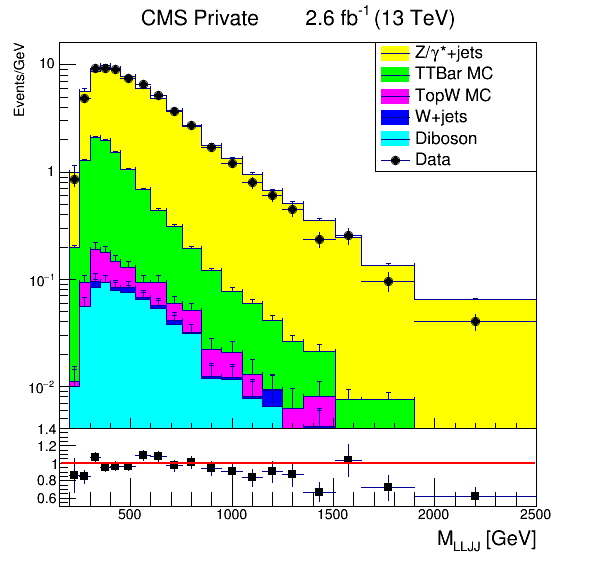
\includegraphics[width=2.4in]{figures/Mlljj_eeChnl_lowMllCR.png}
	\end{subfigure}
	\thickspace
	\begin{subfigure}[t]{2.4in}
		\centering
		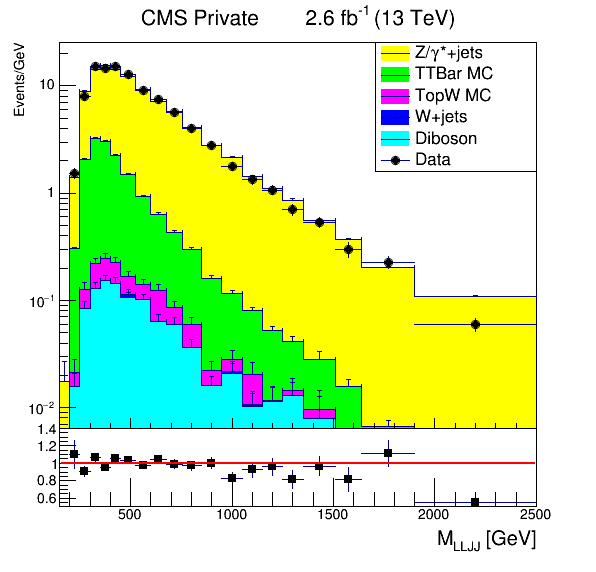
\includegraphics[width=2.4in]{figures/Mlljj_mumuChnl_lowMllCR.png}
	\end{subfigure}
	\caption{The $\Mlljj$ distributions from data and simulated background events that passed the low $\Mll$ control region selection 
		criteria.  The $ee$-channel is on the left, and the $\mu\mu$-channel on the right.  The bin widths are variable, and the bin 
	contents are normalized to their widths.}
	\label{fig:mlljjLowMllCR}
\end{figure}

Initially the large shape discrepancy was attributed to a limitation of the $\DY$+jets simulation - the \DY interaction was simulated 
at leading order in the electroweak and QCD couplings.  This hypothesis was tested by simulating a separate set of 
$\DY$+jets events using a different \MC generator at next-to-leading order in the electroweak and QCD couplings, and with up to four 
radiated partons leaving the \DY interaction.  Then, the procedure described in Section \ref{sec:dyNormInMlljj} was repeated to 
calculate a $\DY$+jets normalization correction for the simulated \DY events.  The normalization correction was applied, and 
simulated $\DY$+jets and other background events were selected using the low $\Mll$ control region selection criteria.  The $\Mlljj$ 
distribution found in simulated events, compared to data in Figure \ref{fig:mlljjLowMllCRAMC}, showed a larger discrepancy with the data 
when using the next-to-leading order $\DY$+jets simulation.  The increased discrepancy was not caused by 
higher order QCD or electroweak interactions, but a significant decrease in selected events.  Comparing the leading order 
and next-to-leading order $\DY$+jets simulations after applying the low $\Mll$ selection criteria, the next-to-leading order simulation 
produced $\sim$3$\times$ fewer events with $\Mlljj > 0.6$ $\TeV$, and $\sim$10$\times$ fewer events with $\Mlljj > 1$ $\TeV$.  Similar 
deficits in selected events were found in events that had $\Mlljj > 600$ $\GeV$ and $\Mll > 200$ $\GeV$.  For these reasons the 
next-to-leading order $\DY$+jets simulation was not used to estimate the $\DY$+jets background, and the large shape discrepancy could not 
be attributed to next-to-leading order effects.

The effect of the 40\% $\Mlljj$ shape discrepancy on the \DY background prediction can be accounted for in two ways.  The simulated $\DY$+jets 
event weights can be adjusted to match the $\Mlljj$ distribution found in data, or an uncertainty can be assigned to the \DY background 
prediction.  Correcting the simulated 
event weights to match the data was not done for two reasons.  First, the variation of the $\Mlljj$-dependent correction versus $\Mll$ could 
not be checked.  This was a significant concern in particular for events that had $\Mlljj > 1900$ $\GeV$, because the weight of those 
events would have been corrected by 40\%.  Second, the uncertainty on the correction was dominated by the statistical uncertainty of the data, 
which exceeded 30\% for $\Mlljj > 1900$ $\GeV$.  Therefore, the $\Mlljj$ distribution found in corrected $\DY$+jets events would still have a 
large uncertainty.  For these reasons, the effect of the 40\% $\Mlljj$ shape discrepancy was accounted for by applying an uncertainty to the 
\DY prediction, whose magnitude was determined as follows.  The results of the search presented here were obtained by counting 
the number of predicted $\DY$+jets events in bins of $\Mlljj$.  Each bin is linked to a specific \mWR hypothesis, and the shape of the \DY 
$\Mlljj$ distribution in each bin is irrelevant.  Thus a shape discrepancy and a normalization discrepancy have the same effect - the total 
number of events in the bin change by the magnitude of the discrepancy.  Therefore, the effect of the 40\% shape discrepancy was accounted for 
by assigning a 40\% uncertainty to the normalization of the $\Mlljj$ distribution found in simulated $\DY$+jets events, independent of $\Mlljj$.

\begin{figure}
	\centering
	\begin{subfigure}[t]{2.4in}
		\centering
		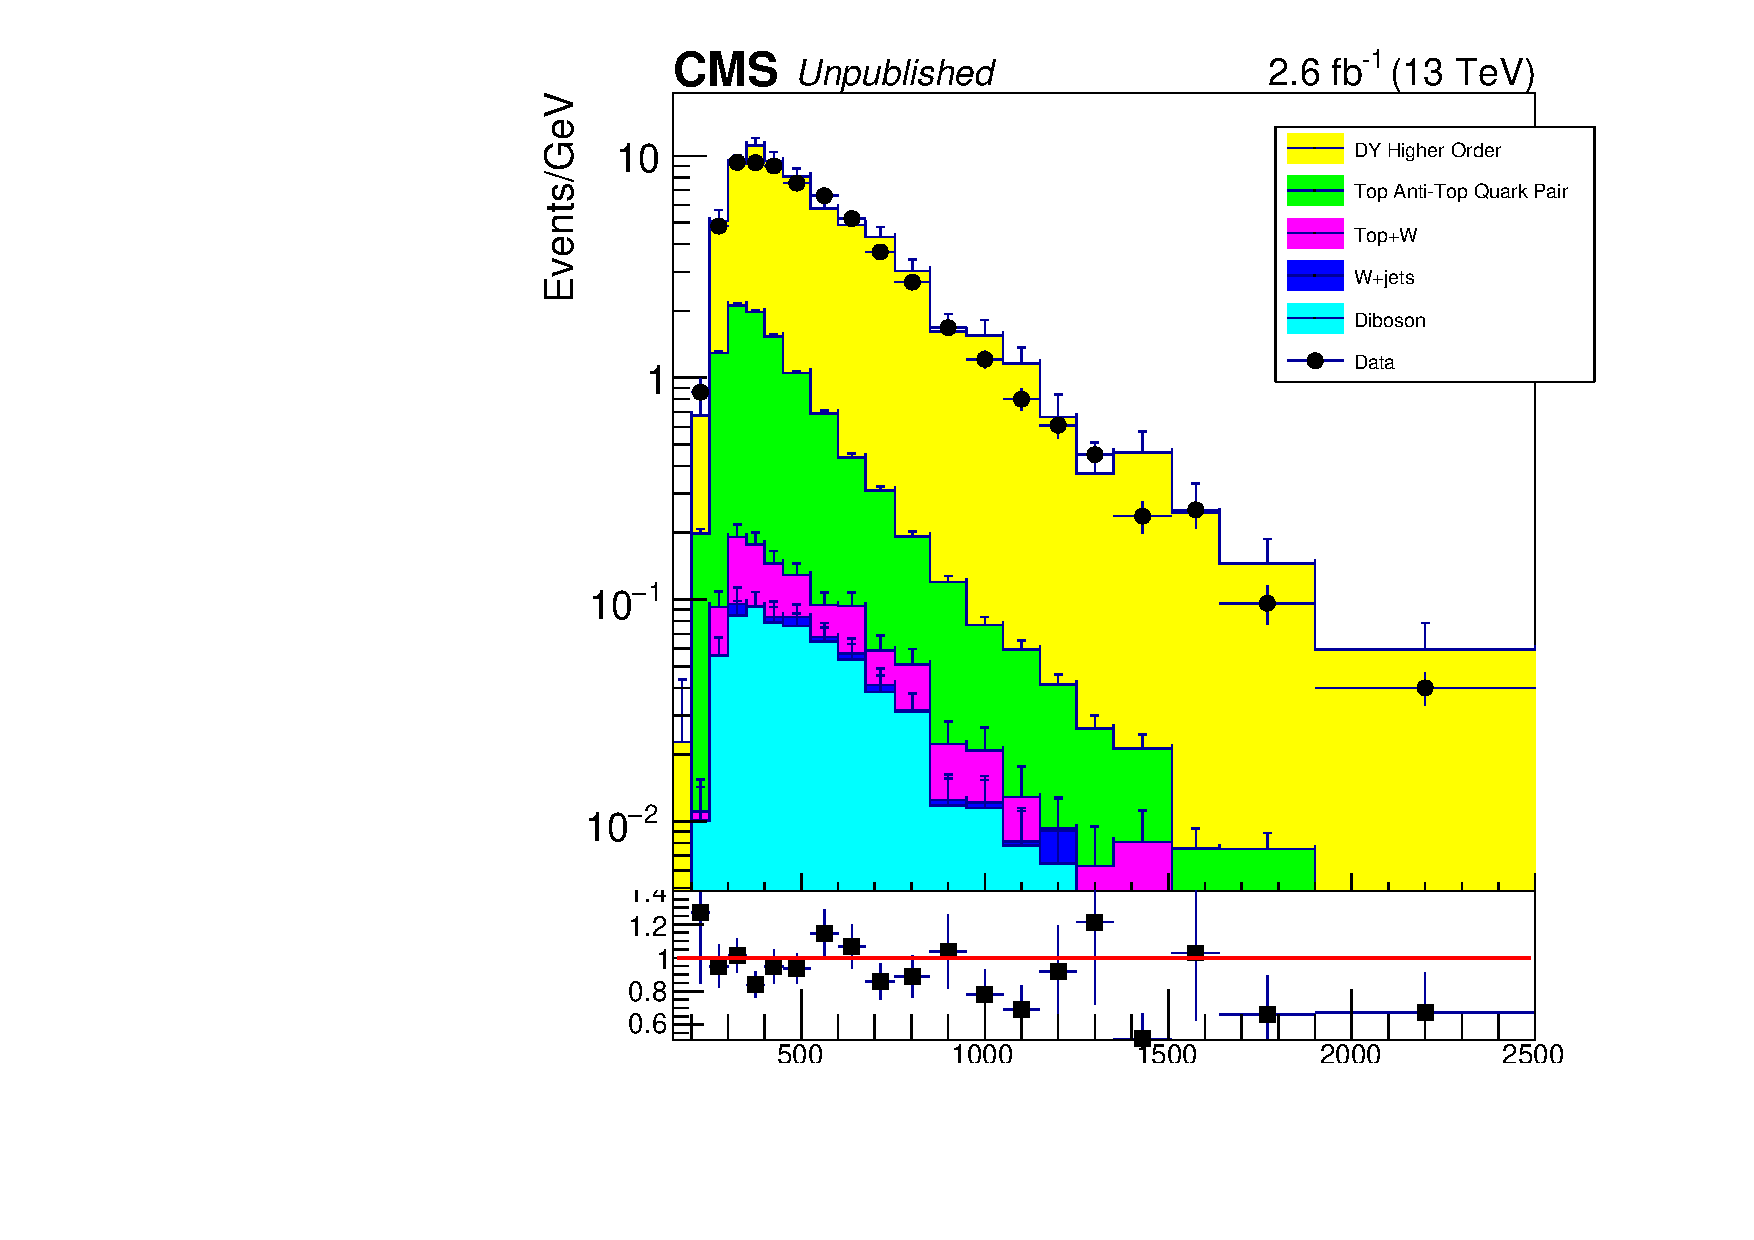
\includegraphics[width=2.4in]{figures/Mlljj_eeChnl_lowMllCR_AMCNLO.pdf}
	\end{subfigure}
	\thickspace
	\begin{subfigure}[t]{2.4in}
		\centering
		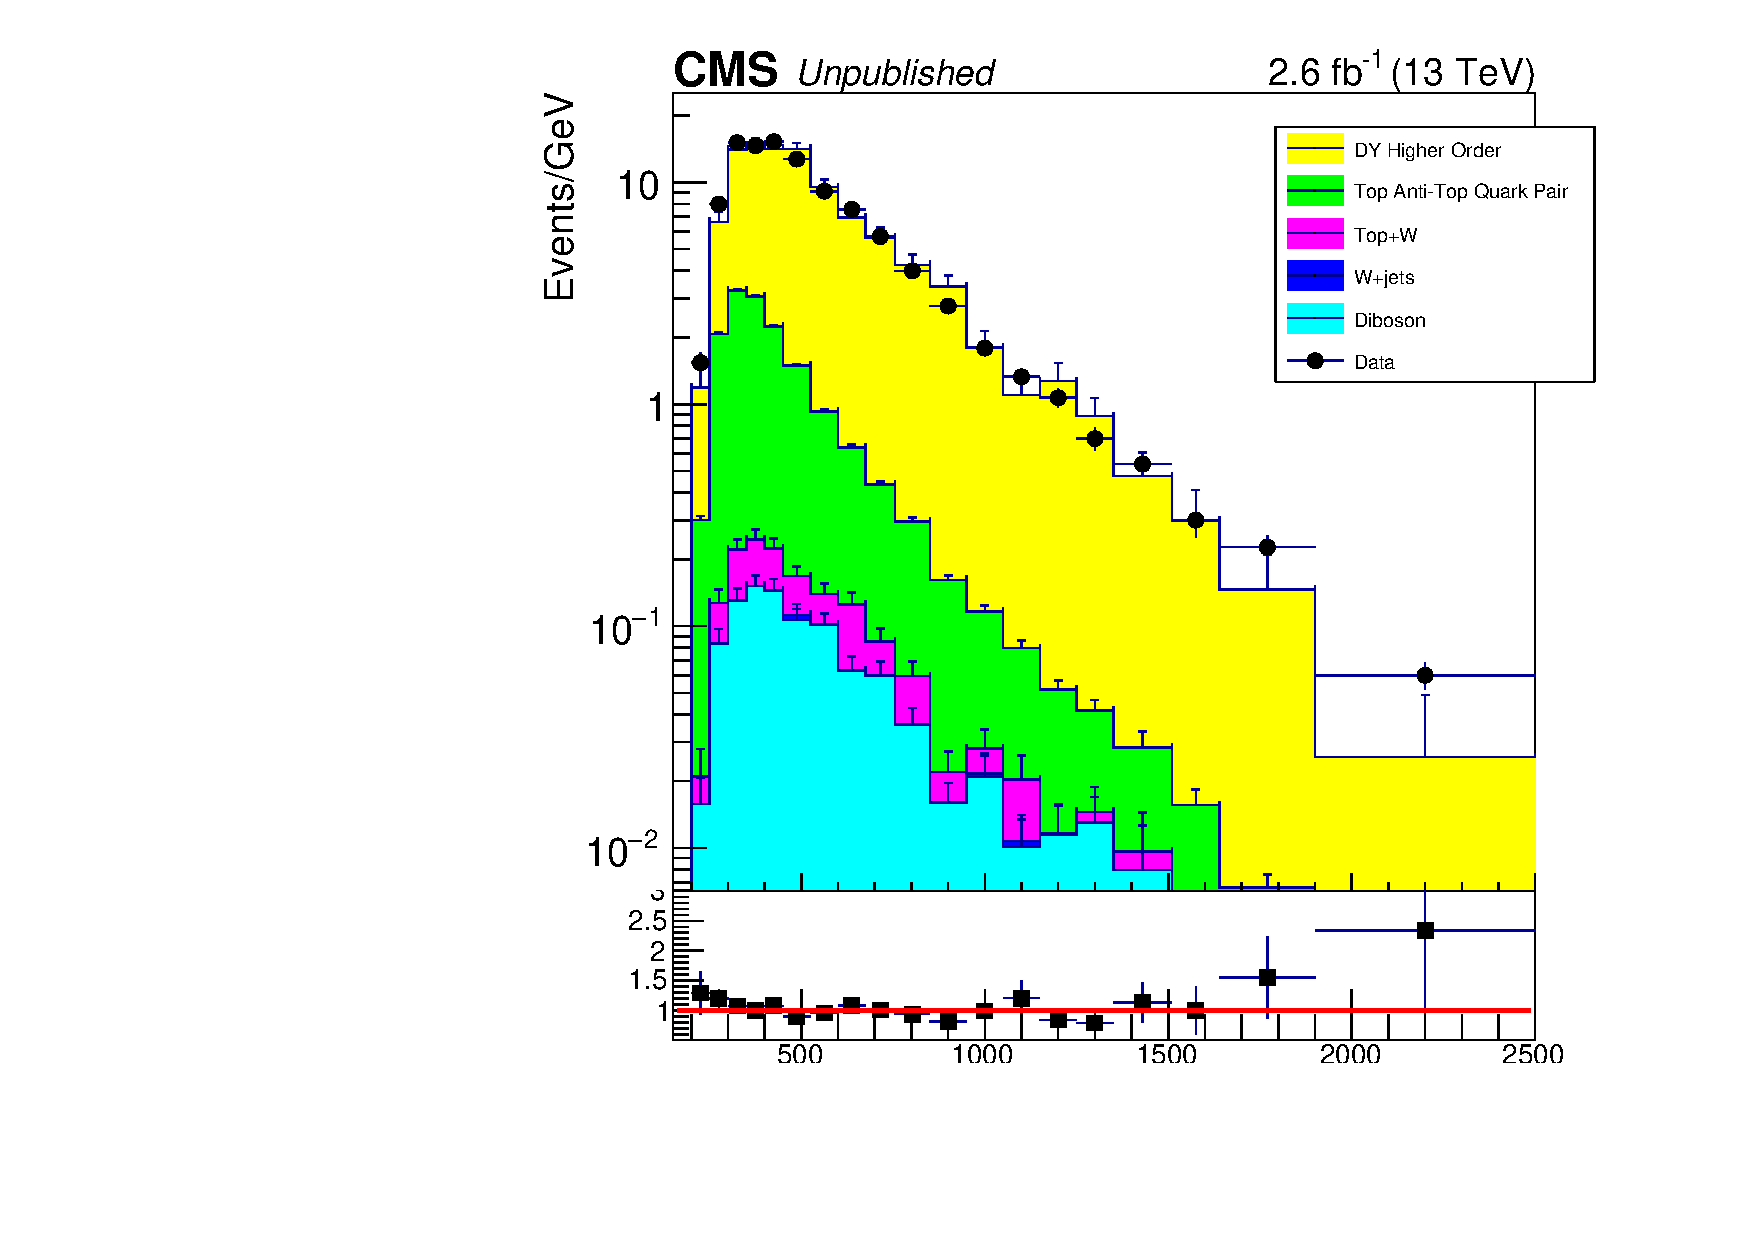
\includegraphics[width=2.4in]{figures/Mlljj_mumuChnl_lowMllCR_AMCNLO.pdf}
	\end{subfigure}
	\caption{The $\Mlljj$ distribution found in data and simulated background events that passed the $\Mll < 180 \GeV$ selection criteria.  
		The $ee$-channel is on the left, and the $\mu\mu$-channel is on the right.  The bin contents are normalized to their widths.}
	\label{fig:mlljjLowMllCRAMC}
\end{figure}

The low $\Mlljj$ control region was used to validate the $\sim$15\% correction applied, and 40\% uncertainty assigned to the predicted 
\DY normalization.  Events from data and all background simulations were selected using the same selection criteria as the low $\Mll$ 
control region, but with $\Mll > 200$ $\GeV$ and $\Mlljj < 600$ $\GeV$.  The weight of simulated \DY events was increased by $\sim$15\%, and 
then the $\Mll$ distributions found in selected data and simulated background events were compared.  The comparison, shown in Figure 
\ref{fig:mllInLowMlljjSideband}, shows that the $\sim$15\% \DY correction brought the background estimate into better agreement with the 
data.  In addition, the 40\% \DY normalization uncertainty was not too conservative, because the disagreement between data and estimated 
backgrounds approached 40\% in several bins.

\begin{figure}
	\centering
	\begin{subfigure}[t]{2.4in}
		\centering
		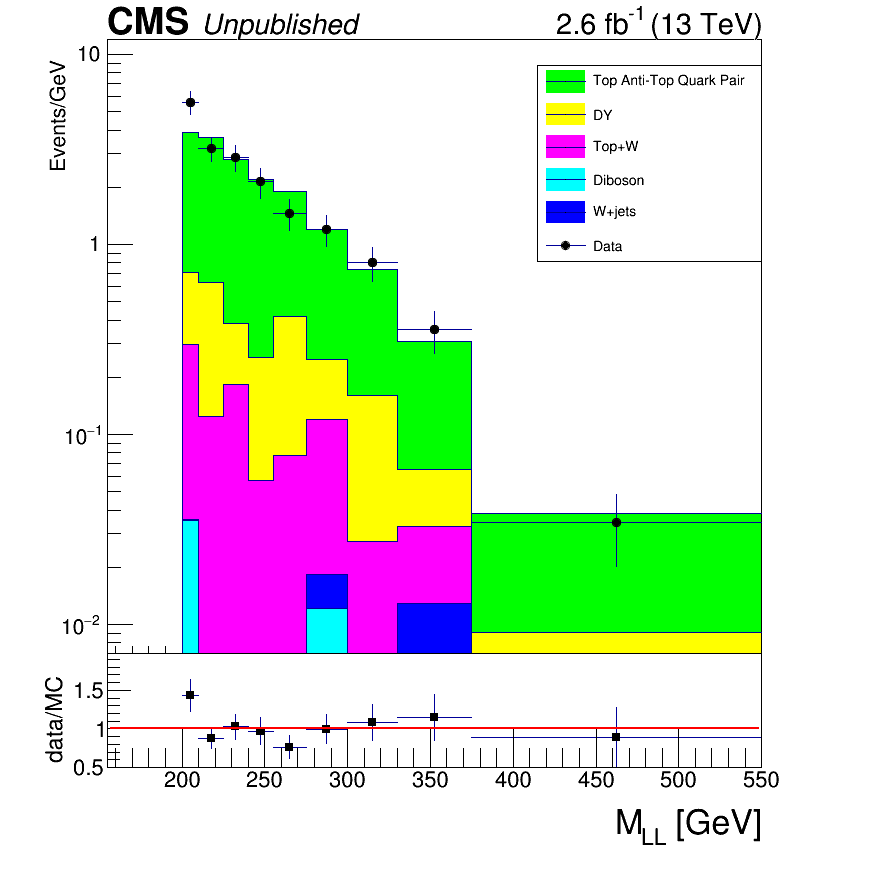
\includegraphics[width=2.4in]{figures/Mll_eeChnl_lowMlljjCR.png}
	\end{subfigure}
	\thickspace
	\begin{subfigure}[t]{2.4in}
		\centering
		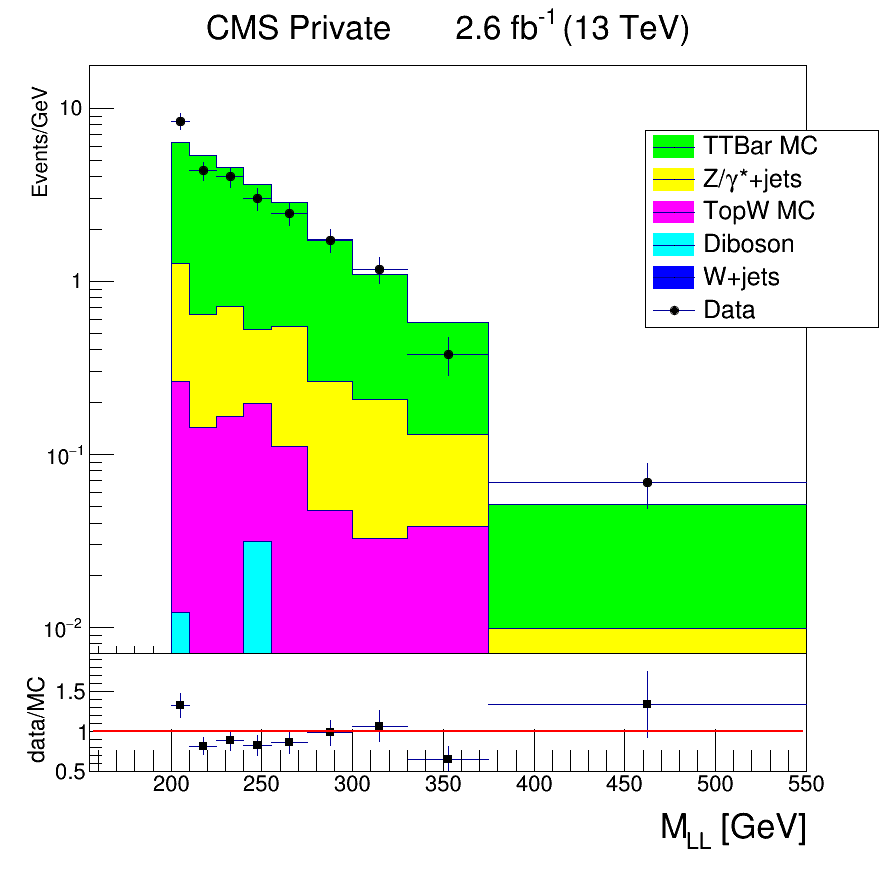
\includegraphics[width=2.4in]{figures/Mll_mumuChnl_lowMlljjCR.png}
	\end{subfigure}
	\caption{The $\Mll$ distribution found in data and simulated background events that passed the low $\Mlljj$ control region 
		requirements.  The $ee$-channel is on the left, and the $\mu\mu$-channel is on the right.}
	\label{fig:mllInLowMlljjSideband}
\end{figure}

\subsection{\DY summary}
The \DY contribution to the $\Mlljj$ distribution found in data was estimated by selecting simulated \DY events using the selection criteria 
described in Chapter \ref{sec:reco_chapter}.  The weight of each selected event was increased by 15.7\% the $ee$-channel, and by 14.2\% in 
the $\mu\mu$-channel.  When calculating the results, a 40\% uncertainty was assigned to the estimated number of \DY events.


\section{Diboson and W+jets Backgrounds}
\label{sec:dibosonAndWJetsBkgnds}
The diboson (WW, WZ, ZZ) and W+jets interactions produced $\ell\ell jj$ events at a much lower rate than the $\DY$+jets interaction.  No 
control region existed where the diboson or W+jets backgrounds could be extracted directly from data, so their contributions to the 
$\Mlljj$ distributions found in data were estimated using simulated events.  The $\Mlljj$ distribution found in selected diboson and W+jets 
events (Figure \ref{fig:allExpectedBkgnds}) was concentrated in the $\Mlljj \leq 2.0$ $\TeV$ region, and its integral was less than 3\% 
of the predicted $\DY$+jets $\plus$ top quark background events.  For these reasons the diboson and W+jets contributions to the $\Mlljj$ 
distribution found in data were neglected.

\begin{figure}
	\centering
	\begin{subfigure}[t]{2.4in}
		\centering
		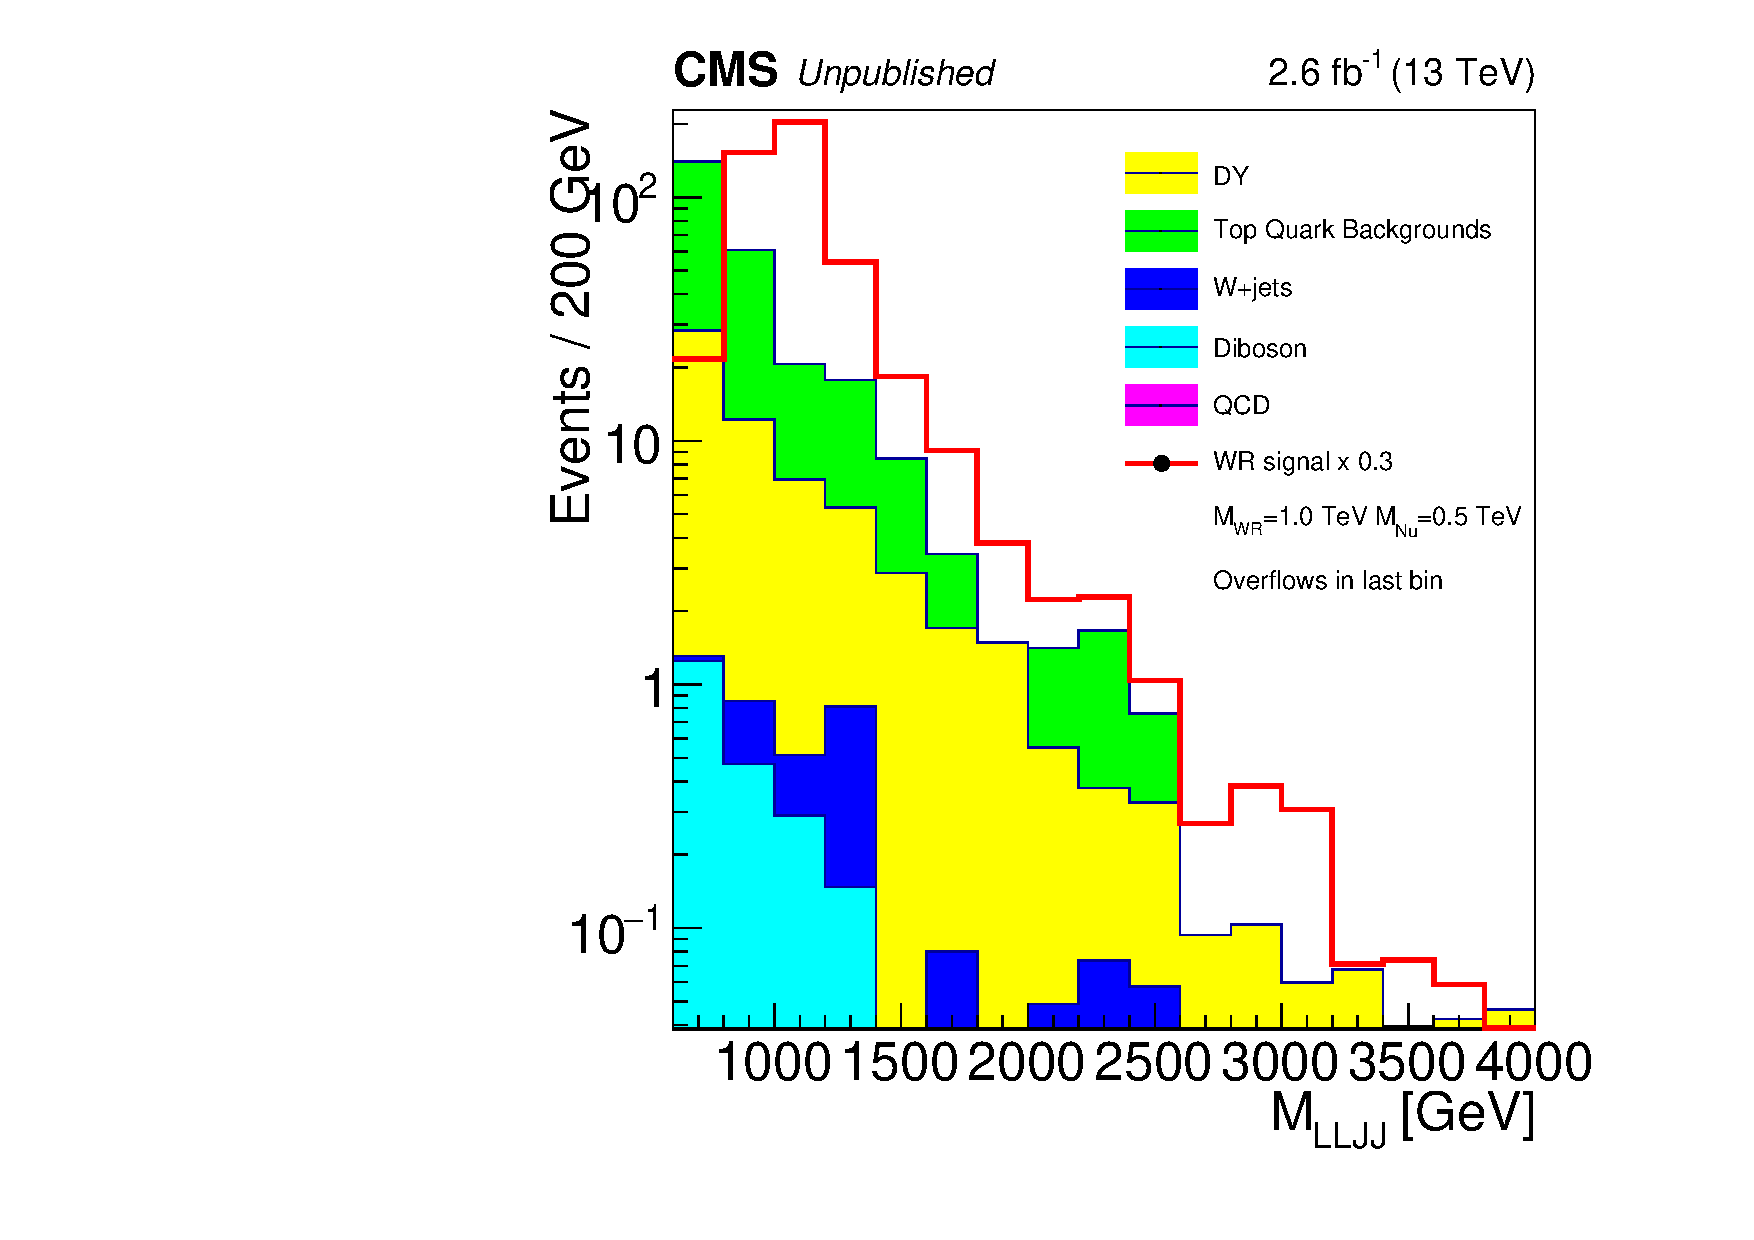
\includegraphics[width=2.4in]{figures/useOfLLJJMassAsFigureOfMerit.pdf}
	\end{subfigure}
	\thickspace
	\begin{subfigure}[t]{2.4in}
		\centering
		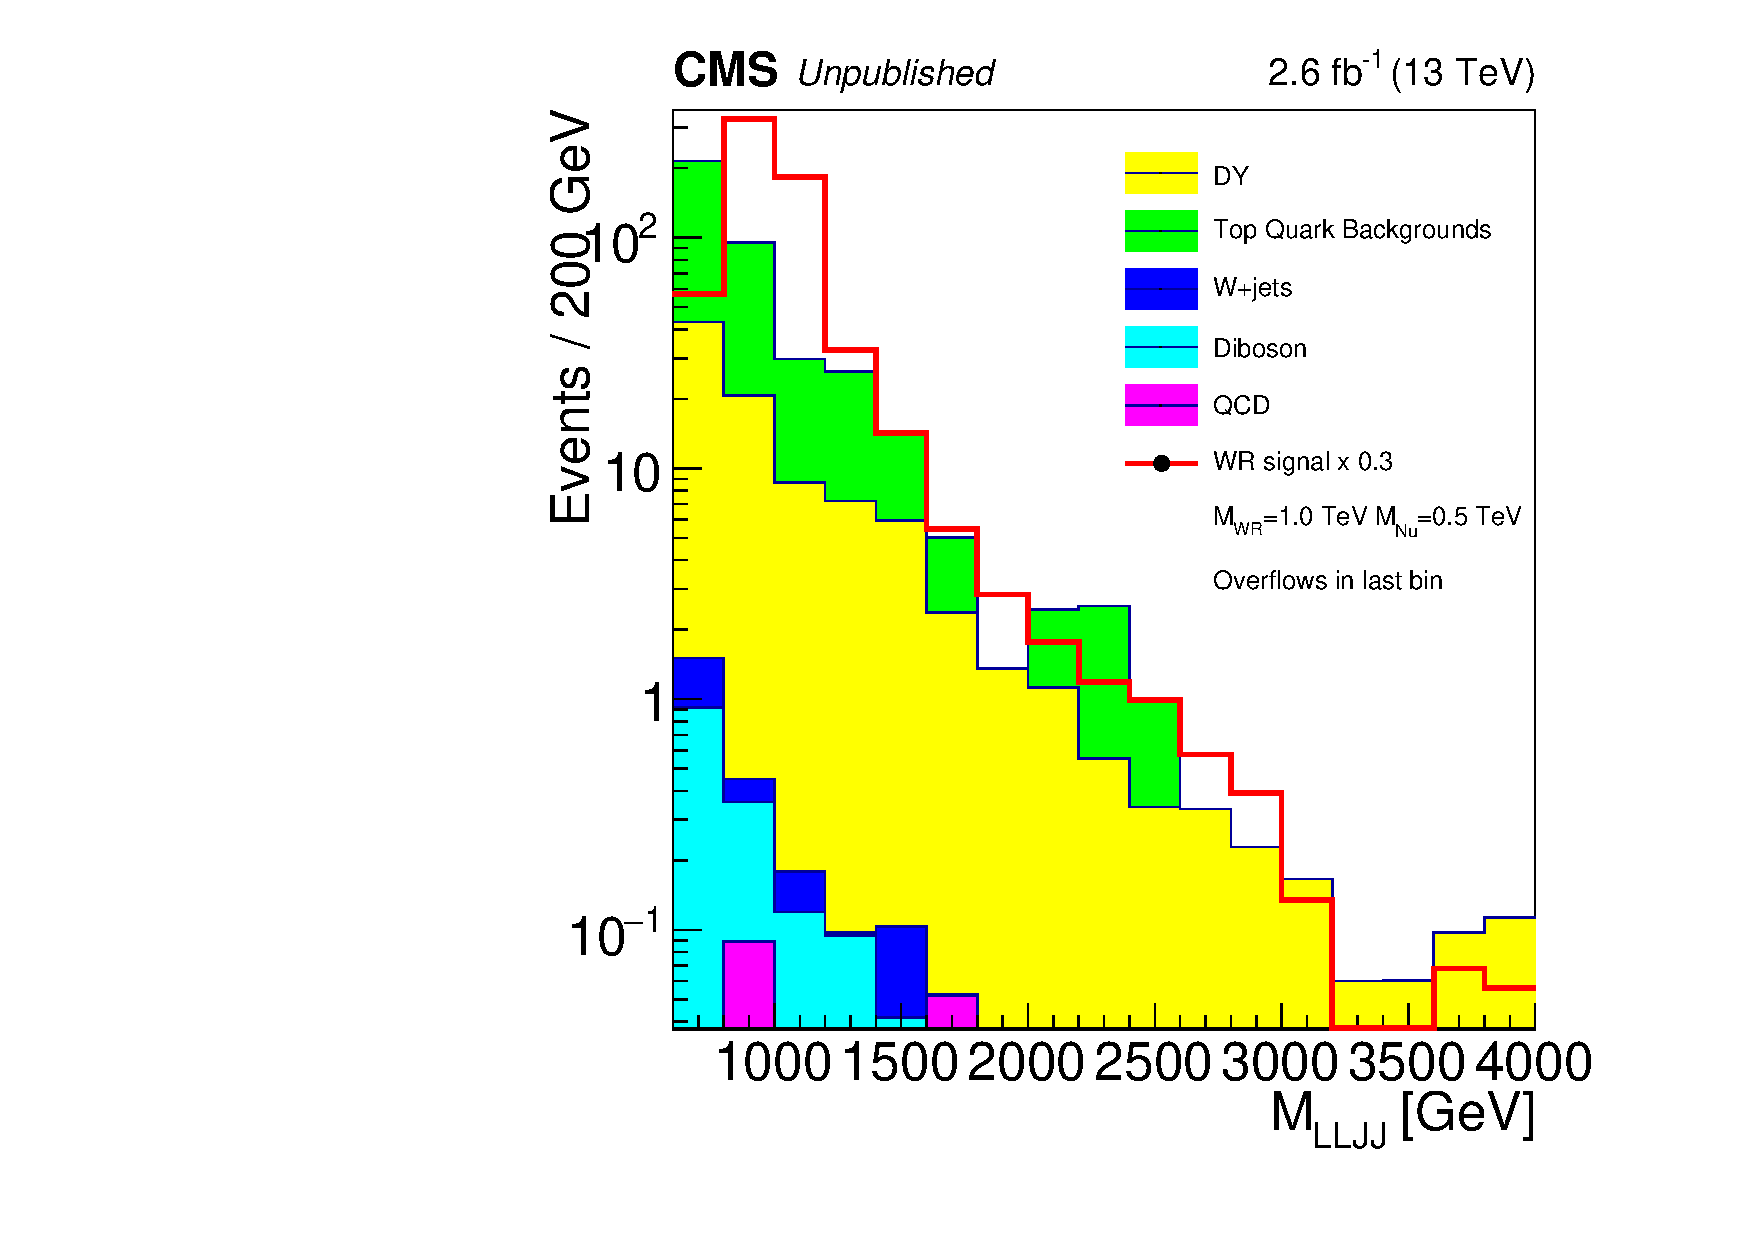
\includegraphics[width=2.4in]{figures/Mlljj_mumuChnl_signalRegionNoData.pdf}
	\end{subfigure}
	\caption{The $\Meejj$ (left) and $\Mmumujj$ (right) distributions found in selected signal and background events.  The top 
		quark and QCD backgrounds are estimated using data. The \WR $\Mlljj$ distribution normalization is reduced by 70\%.}
	\label{fig:allExpectedBkgnds}
\end{figure}


\section{QCD Background}
\label{sec:qcdBkgnd}
Similar to the diboson and W+jets interactions, QCD multi-jet interactions produced $\ell\ell jj$ events at a much lower rate than the 
$\DY$+jets interaction.  Unlike the other backgrounds, the leptons selected offline in QCD events were incorrectly reconstructed from 
jets that contained energetic electrons or photons.  Events in data where two jets may have been identified as leptons were selected 
using the online and offline selection criteria described in Chapter \ref{sec:reco_chapter}, but using the following (reduced) lepton 
ID selection criteria:

\textbf{Muons}
\begin{itemize}
	\item The silicon tracker track was reconstructed from signals in at least 1 silicon pixel detector layer, and signals in at least 
		5 layers in the entire tracker.
\end{itemize}

\textbf{Electrons}
\begin{itemize}
	\item The electron track was reconstructed from signals in every silicon pixel and inner strip detector layers, or all but 1 layer.
	\item The electron track's origin was separated from its vertex by a small distance $\Delta_{xy}$ in the $x-y$ 
		plane: $\Delta_{xy} < 0.2$ mm in the tracker barrel, and $\Delta_{xy} < 0.5$ mm in the tracker endcap.
\end{itemize}

Events were rejected if one or both selected leptons passed the standard lepton ID selection criteria.  In the selected events, 
the $\pt$s and $\eta$s of both selected leptons were used as inputs to a $\pt,\eta$-dependent probability function.  This function, 
derived elsewhere \cite{ZprimeRunOneAndTwo}, calculates the probability that a jet reconstructed as a lepton will pass the standard lepton 
ID selection criteria\footnote{The form of the function differed for electrons and muons.}.  The probability calculated for both selected 
leptons was applied to each selected event as a weight.  The $\Mlljj$ distribution found in selected weighted events (Figure \ref{fig:allExpectedBkgnds}) 
was negligible compared to other backgrounds, so the QCD background was neglected.

\section{Background Estimation Summary}
ST interactions produced events in data where two leptons and jets were reconstructed, and passed the selection criteria that was 
designed to select $\WR \rightarrow \ell\ell jj$ events.  The $\Mlljj$ distribution produced by each interaction, and the uncertainty on 
its normalization was estimated using data and simulated events in control regions.  The $\DY$+jets and top quark interactions produced 
more than 97\% of predicted background events, so the sum of the \DY and top quark backgrounds was identified as the total predicted 
background.  The predicted background was compared to data in bins of $\Mlljj$ that were linked to specific \mWR hypotheses.  These bins 
and the comparison between the data and predicted background is discussed in the next chapter.


%%%%%%%%%%%%%%%%%%%%%%%%%%%%%%%%%%%%%%%%%%%%%%%%%%%%%%%%%%%%%%%%%%%%%%%%%%%%%%%%
